\chapter{Grundlagen}

\section{Content Management Systeme}
\subsection{Web Content Management Systeme}
\subsection{Content Management Life Cycle}
\subsection{Anforderungen an Content Management Systeme in der Zukunft}


\section{Entwicklung mit Ruby on Rails}

2004 arbeitete der dänische Programmierer David Heinemeier Hansson an der Umsetzung eines webbasierten Projektmanagement-Tools mit dem Namen Basecamp\footnote{Projekt-Homepage: \href{http://basecamphq.com/}{http://basecamphq.com/}}. Die bei der Realisierung des Projektes umgesetzten Teilkomponenten extrahierte er später und veröffentlicht sie 2005 als Framework unter dem Namen Ruby on Rails.
\newline
\newline
6 Jahre später beschreibt sich das Ruby on Rails Framework selbst mit folgenden Worten:
\begin{quote}
Ruby on Rails is an open-source web framework that’s
optimized for programmer happiness and sustainable
productivity. It lets you write beautiful code by
favoring convention over configuration.
\end{quote}

Die Aussage bezieht sich dabei auf viele Ansätze und Entwicklungsabläufe, die innerhalb des Frameworks umgesetzt werden.
Im folgenden Abschnitt sollen daher die wichtigsten Prinzipien, Paradigmen und Programmierabläufe des Frameworks zusammengefasst werden, um auf dieser Grundlage eine konzeptionelle und programmiertechnische Betrachtung in Kapitel 4 zu ermöglichen.
\newline
\newline
Für eine umfassende Einführung in Rails werden \cite{RubyMetaprogramming2010} und \cite{EnterpriseRails} empfohlen.

\subsection{Don't-Repeat-Yourself}
Zur Optimierung der Entwicklungvorgänge innerhalb des Frameworks propagiert Rails den Grundsatz des DRY (Don't-Repeat-Yourself). Dabei sollen Redundanzen, d.h. die wiederholte Angabe identischer Informationen jeglicher Art vermieden werden. So kann sichergestellt werden, dass sich Änderungen an einer zentralen Stelle im System (z.B. Quellcode) in der gesamten Anwendung auswirken und Duplikate nicht mehrfach angepasst werden müssen.
\subsection{Convention over Configuration}
Viele Web Application Frameworks müssen vor ihrer Nutzung erst mit Hilfe zahlreicher Konfigurationsdateien und endloser Parametereinstellungen zu einem lauffähigen Gesamtsystem zusammengebaut werden\footnote{Rails bezeichnet diese Art der Frameworks mit ihrem Konfigurations-Overhead oft als \emph{enterprisy}. Dies bedeutet jedoch nicht, das Rails für Anwendungsumsetzungen im Enterprise-Bereich ungeeignet ist. Matt Aimonetti stellt dies im Artikel \cite{enterprisy} heraus.}. Abbildung \ref{spring} zeigt beispielhaft solch eine Konfigurationsdatei innerhalb des Java Application Frameworks Spring:

\lstinputlisting[label=spring,language=XML, caption=Konfigurationsdatei im Java Spring Framework]{code/spring.xml}

Um diesen zusätzlichen und zeitraubenden Aufwand vor der eigentlichen Arbeit mit einem Framework zu vermeiden, definiert das Rails Framework zahlreiche Konventionen, die es erlauben, sofort mit der Entwicklungsarbeit zu beginnen. U.a. werden folgende Festlegungen getroffen:

\begin{itemize}
\item
Informationen zur Datenbankverbindung der Anwendung müssen in der Datei database.yml im Unterordner config hinterlegt werden
\item
Der Klassenname eines Domainenmodells wird im Singular erwartet, der dazu korrespondierende Tabellename in der Datenbank hingegen im Plural z.B. Domainenmodell Project => Datenbanktabelle projects
\item
Der Primärschlüssel in einer Datanbanktabelle muss vom Typ Integer sein und den Namen ID besitzen
\item
Rails erwartet eine definierte Ordnerstrukur für Controller, Domainmodell und Views\footnote{Eine Erklärung zu Model-View-Controller folgt in Abschnitt \ref{sec.mvc}}
\end{itemize}
Für den produktiven Einsatz des Frameworks müssen diese daher erlernt und akzeptiert werden, was dazu führt, dass Rails häufig als \emph{opinionated software\footnote{Eine ausführliche Stellungnahme von David Heinemeier Hansson zu diesem Thema gibt es unter: \href{http://www.linuxjournal.com/article/8686}{http://www.linuxjournal.com/article/8686}}} bezeichnet wird.

Ein Abweichen von den definierten Konventionen ist jederzeit möglich, erhöht jedoch den Aufwand des Entwicklers.

\subsection{Model-View-Controller}
\label{sec.mvc}
Das Ruy on Rails Framework baut wie andere Web-Frameworks auf einem Mehr-Schichten-Architektur-Modell auf. Zusätzlich kommt das bereits 1979 von dem Norweger Trygve Mikkjel Heyerdahl entwickelte Model-View-Controller-Paradigma zum Einsatz.
Die folgende Abbildung charakterisiert dabei den rails-internen Ablauf einer Anfrage innerhalb des Client-Server-Modells:

\begin{figure}[!h]
\begin{center}
\label{sec.mvc}
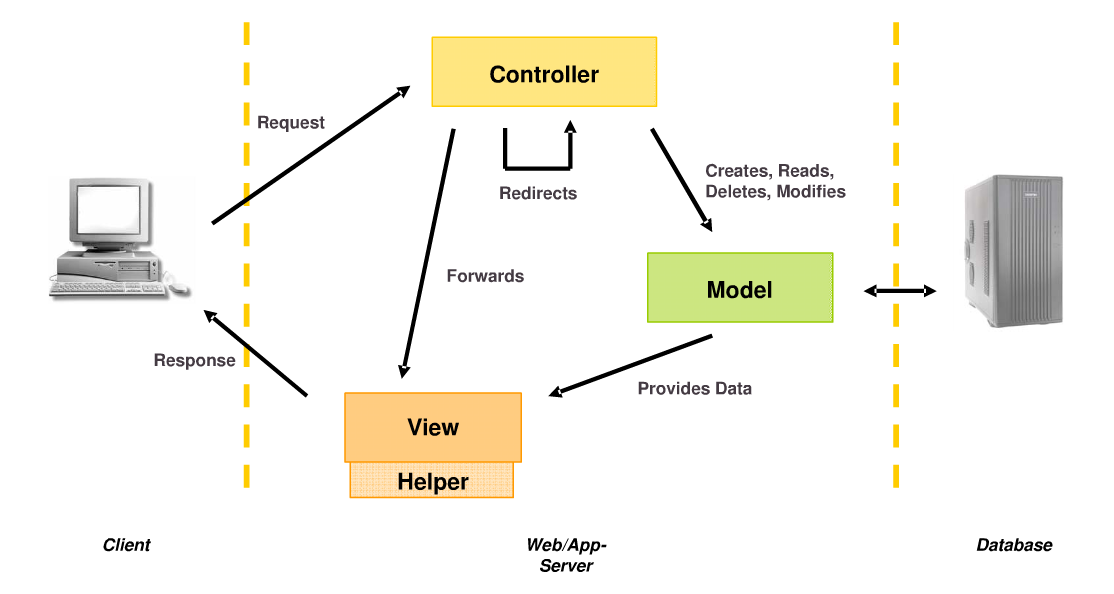
\includegraphics[scale=0.4]{images/analyse/mvc.png}
\caption{Abläufe innerhalb des Rails-Frameworks}
\end{center}
\end{figure}

\begin{enumerate}
\item
Anfrage eines Clienten
\item
An Hand der im Rails-Routing definierten Einträge wird die Anfrage eines Clienten an den registrierten Controller weitergeleitet
\item
Der Controller greift über ein Model auf benötigte Daten in einem Speicher (z.B. realtionale Datenbank) zu und stellt diese dem View-Layer zur Verfügung. Es ist auch möglich, dass der Controller die Anfrage an einen anderen Controller weiterleitet (Redirects).
\item
Das Model ist in Rails
\item
Der View-Layer bereitet die durch den Controller zur Verfügung gestellten Daten an in der angeforderten Darstellungsform auf. So wird z.B. eine HTML- oder XML-Datei erzeugt.
\item
Das Ergebnis der Anfrage (die Ausgabe des View) wird vom Framework an den Server und von dort an den Clienten gesendet. Der Kommunikationsprozess mit dem Rails-Framework ist damit abgeschlossen.
\end{enumerate}



\subsection{REST}
Innerhalb einer Web-Applikation erfolgt der Austausch zwischen Server und Client durch die Nutzung des HTTP-Protokolls. Dabei wird eine Anfrage (Request) an einen Server geschickt, bearbeitet und eine entsprechende Antwort (Response) mit den angeforderten Inhalten zurückliefert. Ein Großteil der Webanwendungen interpretiert dabei die im HTTP-Protokoll definierten Methoden GET und POST:

\begin{description}
\item[GET]
	Anforderung an den Server, eine über die Adresszeile des Browsers angegebene Ressource zurückzuliefern. Es können zusätzlich Argumente an die angeforderte URL angehängt werden.
\item[POST]
	Mit Hilfe dieser Methode ist es möglich,  große Datenmengen aus z.B. Formularen an einen Webserver zu verschicken. Die übergebenen Informationen werden dabei im sogenannten Body der Anfrage codiert mitverschickt und somit im Vergleich zu GET nicht in der URL sichtbar\footnote{Ein Post-Request findet vor allem bei der Übermittlung von Formularen innerhalb eines Browsers Verwendung.}.
\end{description}


REST, ein Akronym für \textbf{RE}epresentational \textbf{S}tate \textbf{T}ransfer, erweitert die in  traditionellen Webanwendungen üblichen GET und POST um die ebenfalls im HTTP-Standard enthaltenen Methoden PUT und DELETE:
\begin{comment}
\begin{description}
\item[GET]
Abfrage einer Ressource unter der angegebenen URL mit  anschließender Darstellung
\item[POST]
Erstellung einer neuen Ressourcen an Hand der in der Anfrage übermittelten Daten, Realisierung durch Formulare auf Clientseite
\item[PUT]
Überschreiben der angeforderten Ressource mit den in der Anfrage neu übermittelten Daten
\item[DELETE]
Löschen der beschriebenen Ressource
\end{description}
\end{comment}

\begin{description}
\item[PUT]
	Die Verwendung der PUT-Methode zeigt die Neuanlage der in einer	Anfrage spezifizierten Ressource an
\item[DELETE]
	Die Verwendung dieser Methode signalisiert dem Server, die angegebene Ressource auf dem Server zu löschen.
\end{description}
Rails unterstützt REST seit der Einführung der Version 1.2 und ermöglicht es so, an Hand einer URL und den verwendeten HTTP-Methoden die richtige Aktion auf dem Server auszuführen. Die URL einer Anfrage repräsentiert damit nicht eine bestimmte Aktion, die beim Aufruf auf dem Server ausgeführt werden soll, sondern eine Ressource\footnote{Der Begriff Ressource bezeichnet in diesem Zusammenhang eine bestimmte Sache.}, die eindeutig zugeordnet werden kann\footnote{Die Eindeutigkeit der Ressource muss vom Entwickler sichergestellt werden.}.
Da aktuelle Browser nur GET- und POST-Anfragen zuverlässig unterstützen, müssen entsprechende Anfragen zum Löschen und Verändern einer Ressource mit Hilfe von zusätzlichen Attributen in der Anfrage simuliert werden\footnote{Das Rails Framework fügt  innerhalb von Formularen automatisch einen versteckten Parameter \emph{\_method} in die Anfrage, die den Namen der gewünschten HTTP-Metode (DELETE oder PUT) enthält. Im Framework wird dieser Parameter ausgelesen und ein entsprechendes Routing zur geforderten Controller-Action eingeleitet}. Das folgende Beispiel stellt das von Rails definierte Standard-Routing einer als \emph{restful} angelegten Ressource Projekt dar\footnote{REST wird nicht über einen entsprechend formulierten Standard definiert. Vielmehr kann es als Programmierparadigma innerhalb von Web-Anwendungen verstanden werden, die eine Ansammlung von Best-Practices darstellen (vgl. \cite{restful}).}.

\begin{table}[!h]
\caption{Standard-Routing für eine Ressource Projekt innerhalb des Rails-Frameworks}
\center
\begin{tabular}[!ht]{|p{2cm}|p{3cm}|p{3cm}|p{6cm}|}
\hline
HTTP-Methode & Anfragepfad & Ausgelöste Aktion im Controller & Wirkung\\
\hline
GET	& /projects & index & Anzeige aller vorhandenen Projekte\\
\hline
GET	& /projects/new	& new &	Anzeige eines HTML-Formulars zum erstellen eines neuen Projektes\\
\hline
POST & /projects & create & Erstellt ein neues Projekt mit den übermittelten Daten\\
\hline
GET & /projects/:id &	show &	Anzeige eines Projektes mit der zugeordneten ID\\
\hline
GET	& /projects/:id/edit & edit & Anzeige eines HTML-Formulars zum Bearbeiten eines bestehenden Projektes\\
\hline
PUT	& /projects/:id &	update & Aktualisierung eines bestimmten Projektes mit den übermittelten Daten\\
\hline
DELETE & /projects/:id &	destroy &	Löschung des Projektes mit der angegebenen ID\\
\hline
\end{tabular}
\end{table}

\begin{table}[!h]
\caption{Vergleich zwischen Rest-konformen und klassischen Rails-URL's}
\label{tab.restnonrest}
\center
\begin{tabular}[!ht]{|l|l|l|}
\hline
Aktion & normale URL & 	REST URL in Rails \\
\hline
show &	/projects/show/12 &	/projects/12 \\
\hline
delete & /projects/destroy/123 & /projects/123 \\
\hline
update & /projects/update/123 &	/projects/123 \\
\hline
create & /projects/create & /projects \\
\hline
\end{tabular}
\end{table}

Tabelle \ref{tab.restnonrest} zeigt noch einmal die Trennung zwischen Ressource und Aktion innerhalb einer in Rails definierten REST-Ressource Projekt. Eine ausführliche Beschreibung von REST und dessen Realisierung liefert \cite{Wirdemann08}.

\subsection{Rack und Middleware}
\subsection{Datenbankgetriebene Entwicklung}
\subsection{Generatoren}

%ANALYSE'####################################################################################'
\newpage

\section{Externer Kriterienkatalog}
Die hohe Zahl am Markt befindlicher Web Content Management Systeme führt zu einem erschwerten Auswahlverfahren. Neben vielen kostenpflichtigen, professionellen WCMS-Lösungen stehen durch die Open Source Bewegung zusätzlich zahlreiche kostenlose Softwareprodukte zur Verfügung, die sich in ihrer Leistungsfähigkeit stark unterscheiden.
So kommt es häufig vor, das klein angelegte Open Source Projekte ihre Software stolz als Web Content Management System bezeichnen, obwohl nur sehr wenige Funktionalitäten implementiert sind.
Um dieser Praktik entgegenzuwirken haben Vertreter der Content Management Branche eine Feature Matrix (Abb. \ref{featurematrix}) herausgegeben, die aktuelle Anforderungen an ein Content Management System spezifizieren soll. Die dabei entstandene Übersicht zeigt dabei eine Unterscheidung in 3 Prioritätsstufen:
\begin{description}
\item[Must-Have]\mbox{~}\\*
Diese Funktionalität muss in einem Content Management System verhanden sein.
\item[Should-Have]\mbox{~}\\*
Diese Funktionalität ist nicht zwingend notwendig, kann bei entsprechender Existenz aber sehr positv wahrgenommen werden.
\item[Nice-to-Have]\mbox{~}\\*
Funktionalitäten, die nur in wenigen, hochwertigen Systemen zur Verfügung stehen und über die gewöhnlichen Anforderungen hinausgehen.
\end{description}


\begin{figure}[!h]
\begin{center}
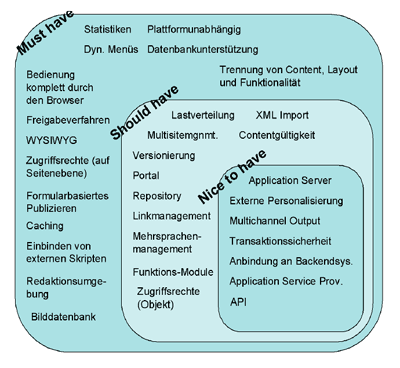
\includegraphics[scale=0.3]{images/analyse/wcmfeaturematrix.png}
\caption{Feature-Matrix für Content Management Systeme}
\label{featurematrix}
\end{center}
\end{figure}


Die beschriebenen Funktionalitäten sind jedoch teilweise so allgemein formuliert, das dieser Ansatz nur als grobe Orientierungshilfe dienen kann.
Der Wirtschaftsinformatiker Andreas Ritter hat daher im Rahmen seiner Bachelorarbeit \emph{SWOT-Analyse zu Content-Management-Systemen} einen Kriterienkatalog erarbeitet, an Hand deren die Leistungsfähigkeit von Web Content Management Systemen untersucht werden kann. Diese orientieren sich dabei an den Prozessen des Content Managements und des Content Life Cycles [Vgl. Rit101].
\newline
\newline
Die von Ritter formulierten Kriterien werden in den Kapiteln 5.3.1 bis 5.3.5 nochmals aufgeführt und bilden die Grundlage für die Bewertung der Leistungsfähigkeit der ausgewählten Ruby on Rails Content Management Systeme.



\subsection{Zielgruppe}
Der externe Kriterienkatalog


\subsection{Erstellung}
\begin{itemize}
\item
Mehrere Benutzer sollen gleichzeitig Inhalte verwalten und erfassen können
\item
Inhalte sollen – unabhängig von Zeit und Standort – durch mehrere Benutzer online verwaltet und erfasst werden können
\item
Für die Verwaltung und Erfassung von Inhalten sollen alle gängigen Internet-Browser (Internet Explorer, Safari und Firefox) eingesetzt werden können
\item
Offline Erfassung von Inhalten unter Verwendung eines lokal auf dem Rechner installierten Programms
\item
Inhalte sollen ohne spezielle Programmier / HTML-Kenntnisse erfasst und verwaltet werden können
\item
Integrierte Mediendatenbank zur Erfassung und Verwaltung von Bildern, Multimedia, Texte, Audio, Videos, usw.
\item
Inhalte (Texte, Bilder, Videos etc.) sollen zentral kategorisiert, erfasst und verwaltet werden können
\item
Inhalte sollen in einer Datenbank gespeichert werden
\item
Inhalte sollen mehrsprachig erfasst und verwaltet werden können
\item
Inhalte können während der Erfassung über eine Preview-Funktion vorab im Design der Webseite angesehen werden
\item
Zuordnung von standardisierten und frei definierbaren Metadaten zu Inhalten (z.B. Autor, Schlüsselwörter, benutzerdefinierte Felder) soll möglich sein
\item
Integration von Inhalten anderer Webseiten, Multimedia, Applikationen, E-Commerce- Tools
\item
Das CMS soll über eine offene API (Programmierschnittstelle) für individuelle Erweiterung verfügen
\item
Inhalte sollen einfach importiert / exportiert werden können - dabei kommen Formate wie z.B. XML zum Einsatz
\end{itemize}



%#### end Erstellung

\subsection{Kontrolle}


\begin{itemize}
\item
Granulares Rechte- und Rollenkonzept für Anwender
\item
Granulares Berechtigungskonzept für einzelne Inhalte, Bereiche, Webseiten
\item
Schutz vor gegenseitigem Überschreiben erfasster Inhalte durch Check in/ Check out- Mechanismen
\item
Versionierung von Inhalten mit Möglichkeit zur Wiederherstellung vorhergehender Versionen
\item
Linküberprüfung: Automatische Prüfung der Gültigkeit von internen und externen Links, mit Möglichkeit zur Korrektur bzw. Benachrichtigung an eine definierte Personengruppe
\item
Mandantenfähigkeit: Mehrfachnutzung des Systems durch verschiedene Parteien mit kompletter Trennung der Daten und Benutzer
\end{itemize}

%######## end kontrolle

\subsection{Freigabe}

\begin{itemize}
\item
Definition von Workflows inkl. mehrstufiger Freigabeprozesse für die Freischaltung von Inhalten
\item
Unternehmensspezifische Bearbeitungsprozesse von Inhalten, sollen über frei definierbare Workflows verwaltet werden können
\item
Möglichkeit für \emph{nicht technische} User den Workflow zu kreieren, verwalten und ändern. Es soll dafür kein Scripting / Programming notwendig sein
\item
Möglichkeit externe Benutzer in Workflows mit einbinden zu können
\end{itemize}

%##### end freigabe


\subsection{Publikation}

\begin{itemize}
\item
Trennung von Inhalt und Design unter Verwendung von Templates
\item
Mehrfachverwendung von Inhalten an verschiedenen Stellen mit unterschiedlichem Layout
\item
Möglichkeit zur Wahl zwischen dynamischer oder statischer Generierung der Seiten / Inhalte
\item
Möglichkeit Inhalte für anderen Webseiten bereitzustellen (XML, Webservice)
\item
Navigationsstrukturen werden automatisch vom CMS generiert, publiziert und verwaltet
\item
Automatisches Anbieten von Druckversionen und Weiterempfehlen einer Webseite
\item
Inhalte sollen auf verschiedene Medien / Technologien (Cross Media Publishing, SMS / Mobile / WAP / usw.) ausgegeben werden können
\item
Einfache Einbindung von Fremdinhalten welche durch Drittanbieter zur Verfügung gestellt werden
\item
Schnittstellenunterstützung in Form von APIs sollen zur Verfügung stehen
\item
Barrierefreiheit bei den publizierten Seiten soll unterstützt werden
\end{itemize}

%############## end publikation

\subsection{Terminierung und Archivierung}

\begin{itemize}
\item
Inhalte sollen archiviert werden können
\item
Freie Wahl des Publikationszeitraumes (zeitgesteuertes Auf- / Abschalten / Archivieren) von Inhalten
\end{itemize}

%############## end terminierung

